\documentclass{article}

% CSCI 566 midterm report. ICML 2026 two-column format, matching the
% pre-proposal. Course instructions override conference defaults: author
% names must be visible -> preprint option. Numeric citations to match the
% pre-proposal's [1], [2] style.
\PassOptionsToPackage{numbers,compress}{natbib}
\usepackage{microtype}
\usepackage{graphicx}
\usepackage{booktabs}
\usepackage{hyperref}
\usepackage[preprint]{icml2026}

% Course report: restore numeric citations [1], [2] to match the
% pre-proposal (the stock style forces author-year at its line 551).
\setcitestyle{numbers,square,citesep={,}}

\usepackage{amsmath}
\usepackage{amsfonts}
\usepackage{array}
\usepackage{placeins}

\setcounter{dbltopnumber}{3}
\renewcommand{\dbltopfraction}{0.85}

\icmltitlerunning{TaskFlow-Travel: Midterm Report}

\begin{document}

\twocolumn[
  \icmltitle{TaskFlow-Travel: Imitation-Learned Coordination for Multi-Agent
    Travel Replanning under Evolving User Constraints\\
    \large Midterm Progress Report}

  \begin{icmlauthorlist}
    \icmlauthor{Chenhao Liang}{usc}
    \icmlauthor{Chenshuhao Qin}{usc}
    \icmlauthor{Kaixiang Liu}{usc}
    \icmlauthor{Yusong Liu}{usc}
    \icmlauthor{Zhuyu Lu}{usc}
    \icmlauthor{Guangyu Hou}{usc}
    \icmlauthor{Chengfeng Tang}{usc}
  \end{icmlauthorlist}
  \icmlaffiliation{usc}{University of Southern California}

  \icmlkeywords{multi-agent systems, imitation learning, language agents, replanning}

  \vskip 0.3in
]

\printAffiliationsAndNotice{}

\begin{abstract}
TaskFlow-Travel learns when to keep an itinerary, ask for clarification,
search, repair a component, or rebuild after a user's constraints change.
We train a small coordinator from a scripted expert using behavior cloning,
trajectory augmentation, and DAgger. Our TravelPlanner-derived benchmark
contains 1{,}420 episodes over 355 queries, plus a multi-component budget-cut
test family. In offline evaluation, BC with augmentation and three DAgger
iterations reaches 99.6\% revision success with 0.72 simulated calls per turn,
about 14\% fewer than cost-aware rules (100\% success, 0.84 calls per turn).
Under a one-call simulated cap, learned variants achieve 97.6--97.9\%,
compared with 79.7\% for cost-aware rules and 98.5\% for the scripted expert.
The combined model makes about 20\% fewer excess edits than cost-aware rules
on multi-component cuts. Recovery after injected mistakes rises from
90.5--95.9\% with plain BC to 99.1--100\% with augmentation. We plan a
versioned public release of the derived dataset and verifier by the final
submission.
\end{abstract}

\section{Progress so far}
\label{sec:progress}

\subsection{Task recap}
Travel planning is rarely a one-shot request. After seeing an itinerary, a
user may lower the budget, require a hotel that allows pets, drop a cuisine,
or decide that convenience matters more than price. Current LLM agents
respond fluently but often forget earlier constraints or regenerate
unaffected parts of the plan
\citep{xie2024travelplanner,oh2025flextravelplanner}. As proposed in our
pre-proposal, TaskFlow-Travel treats each revision as a coordination
decision: after every update, a coordinator chooses among twelve actions
(\textsc{KeepPlan}, \textsc{AskClarification}, three \textsc{Search} actions,
five \textsc{ReplanLocal}/\textsc{ReplanGlobal} actions, \textsc{Verify},
\textsc{Stop}). The research question is whether this coordination policy can
be \emph{learned by imitation} rather than hand-written, and whether it saves
unnecessary replanning and LLM calls at equal success. A plan is a 13-slot
structure (2 transport legs, 1 stay, 6 meals, 4 attractions); ``do the
minimum'' means changing as few slots as any valid repair requires.

\subsection{What has been built}
All components below are implemented, tested (94 offline tests), and
reproducible. Datasets rebuild byte-for-byte from a fixed seed, and all 18
models retrain to identical weights.

\textbf{Benchmark and verifier.} We parse TravelPlanner's per-query database
slices (flights, ground transport, hotels, restaurants, attractions) and
verify plans with TravelPlanner-style commonsense and hard constraints, plus
our rating floor and cost/quality priority. All 3{,}054 passing expert plans
pass the adapted upstream checks. Queries are split
train/validation/test \emph{before} generating update variants, so no trip
variant crosses splits: 355 three-day single-city queries (215/71/69) expand
into 1{,}420 episodes of 1--4 updates from four types (add, delete, replace,
reprioritize) over seven constraint targets (budget, room type, house rule,
cuisine, transport rule, restaurant rating floor, cost/quality priority).
About 19\% of test turns are infeasible and require clarification, and 63\%
of feasible updates invalidate the plan the coordinator would
otherwise keep (generator target 75\%). The test split is held out three
ways: unseen trips, a second phrasing template set, and 4-turn chains
(training uses at most 3). A one-turn multi-component family (budget cuts
needing 0--3 component changes, 138 test episodes) and a 12-case stress suite
complete the task suite; all 3{,}667 feasibility labels agree with an
independent exact solver.

\textbf{Multi-turn environment and agents.} A rule-based constraint tracker
converts each user message to a structured diff (an LLM tracker with schema
validation and fallback is implemented behind a provider switch).
Deterministic component planners implement local repair (other components
frozen) and global regeneration; LLM-backed variants choose from validated
shortlists. Cached searches go stale when a relevant constraint changes; the
system acts on its own constraint belief, with ground truth used only for
scoring.

\textbf{Coordinators.} Five exist: always-regenerate (plus a deterministic
control), static rules, a \emph{cost-aware} static baseline added after
review (repair components in order of potential savings, ask when even the
cheapest options break the budget), a privileged scripted expert that
searches repairs of up to three components, and an LLM coordinator that
doubles as the DAgger teacher.

\textbf{Learned coordinator.} An MLP over ${\sim}96$ non-privileged
features, trained with behavior cloning (BC), trajectory augmentation, and
DAgger (1--3 iterations), 3 seeds each; 18 models are committed.

\textbf{Evaluation and demos.} All proposal metrics (final pass, revision
success, constraint retention, preservation, LLM/tool calls), an exact
minimum-edit oracle, budget-capped comparisons, forced-mistake recovery,
per-type/turn/level breakdowns, and figures. A local interactive web app
plans trips on supported city pairs and revises them from user messages,
showing four coordinators side by side. The
\href{https://onetrickollie.github.io/taskflow-travel/}{project website}
publishes documentation, results, and recorded replays. CI runs the
offline tests and rebuilds the site on pushes to \texttt{main}.

\subsection{Progress against the pre-proposal}
Table~\ref{tab:vsproposal} maps the pre-proposal to the midterm snapshot.
The static multi-agent baseline is implemented in two variants, and the
learned coordinator is trained. The midterm LLM components were exercised
with offline stand-ins. Section~\ref{sec:plan} schedules the single-agent
baseline and live evaluation. Flex-TravelPlanner is a stretch goal pending
a license check.

\textbf{Response to the pre-proposal review.} The review raised two points,
and both shaped the work so far. First, it flagged \emph{cascading trajectory
error} (distribution shift) as the key technical risk of behavior cloning
for agent coordination, and recommended DAgger or trajectory augmentation
during dataset construction rather than relying solely on offline teacher
cloning. We implemented both: trajectories are augmented with
near-miss and perturbed states, and DAgger iterations re-label the learner's
own states with the expert. Section~\ref{sec:results} measures the concern
directly: forced-mistake recovery rises from 90.5--95.9\% (plain BC) to
99.1--100\% with augmentation. Second, the review asked for a public release
of the evolving-constraint dataset and verifier as a community benchmark.
We plan to publish a versioned release of our derived tasks and verifier by
the final submission, with a dataset card, TravelPlanner attribution, and
reproduction instructions (Section~\ref{sec:plan}).

\begin{table*}[t]
\centering
\caption{Pre-proposal commitments vs.\ status at midterm.}
\label{tab:vsproposal}
\small
\begin{tabular}{@{}>{\raggedright\arraybackslash}p{0.34\textwidth}>{\raggedright\arraybackslash}p{0.58\textwidth}@{}}
\toprule
\textbf{Pre-proposal item} & \textbf{Status at midterm} \\
\midrule
Constraint taxonomy, verifier, leakage-safe splits &
Done; upstream-compatible checks; exact-solver-validated labels \\
Single-agent LLM baseline & Planned (P0; Section~\ref{sec:plan}) \\
Static multi-agent baseline & Done, in two strengths (rules; cost-aware) \\
Learned coordinator (BC) & Done; extended with augmentation and DAgger \\
Real-LLM tracker/agents/coordinator & Implemented and tested with offline
stand-ins; live validation planned (P0) \\
Evolving-constraint tasks from TravelPlanner & Done (v0 $+$ multi-component
family) \\
Flex-TravelPlanner integration & Pending a license check \\
Metrics: success, retention, preservation, cost & Done; plus exact
minimum-edit scoring, budget caps, forced-mistake recovery \\
\bottomrule
\end{tabular}
\end{table*}

\section{Literature review}
\label{sec:litreview}

\textbf{Benchmarks for tool-using travel agents.}
TravelPlanner~\citep{xie2024travelplanner} provides public databases, tools,
and annotated plans for one-shot itinerary generation with commonsense and
hard constraints, and shows that strong LLM agents often fail budget and
constraint checks. Flex-TravelPlanner~\citep{oh2025flextravelplanner} makes
the setting multi-turn: constraints are revealed over several queries, and
models frequently satisfy a new preference while silently breaking an
earlier global constraint such as budget. Our benchmark deliberately goes
beyond constraint \emph{addition}: we generate add, delete, replace, and
reprioritize updates over seven targets, with infeasible updates mixed in,
so the correct action distribution includes asking and keeping silent, not
only repairing. Both works score final plans; we additionally score the
\emph{process}---how many slots were edited beyond the exact minimum---which
is the quantity our coordinator is meant to control.

\textbf{Multi-agent LLM systems.} General frameworks such as
AutoGen~\citep{wu2023autogen} and MetaGPT~\citep{hong2024metagpt} organize
LLMs into conversational or role-specialized societies, and
ReAct~\citep{yao2023react} interleaves reasoning with tool calls for a
single agent. For travel specifically, ATLAS~\citep{choi2025atlas}
decomposes planning into constraint-aware collaborating agents, and
HiMAP-Travel~\citep{bui2026himaptravel} uses hierarchical multi-agent
planning for long constrained itineraries. These systems fix the
\emph{workflow} by hand: which agent acts, in what order, and when to redo
work. TaskFlow-Travel asks the complementary question---given a modular
agent team, can the \emph{dispatch decision} itself be learned from an
expert's demonstrations, and does that beat hand-written dispatch at equal
or lower cost?

\textbf{Imitation learning.} Behavior cloning from expert demonstrations is
the classic approach~\citep{pomerleau1991alvinn}, but errors compound over
long horizons: a policy that strays from the expert's state distribution has
no supervision for recovery~\citep{ross2010efficient}. DAgger fixes this by
aggregating expert corrections on states visited by the
learner~\citep{ross2011dagger}. Recent work uses agents' early environment
interactions as supervision for LLM tool use~\citep{zhang2026earlyexperience}.
Our coordinator is an MLP over a compact state encoding trained with BC,
trajectory augmentation, and DAgger with the scripted expert. We use
forced mistakes to measure recovery (Section~\ref{sec:results}).

\textbf{Plan repair versus replanning.} Classical planning distinguishes
repairing a plan from recomputing one, and shows that minimizing change to a
validated plan is itself a criterion worth
optimizing~\citep{fox2006planstability}. Itinerary regeneration consumes
more calls under our cost model and can discard choices that the user
has accepted. Our edit-optimality metric quantifies unnecessary changes
in conversational replanning.

\textbf{Positioning.} To our knowledge, no prior work learns the
coordination policy of a multi-agent travel planner under genuine constraint
\emph{revision} (including deletions and reprioritization). The closest
systems hand-code dispatch; the closest learning work targets one-shot
tool-use policies rather than repair-versus-rebuild decisions across turns.

\section{Initial results}
\label{sec:results}

\textbf{Setup.} The offline evaluation uses a rule-based tracker and
database-backed planners. A fixed cost model assigns four calls and
6{,}000 tokens to a global rebuild, and one call and 1{,}500 tokens to a
local repair. The main benchmark is the v0 test split (276 episodes,
689 turns). For learned systems we report means over three training seeds
and show standard deviations for success rates when nonzero. A feasible
revision succeeds if its plan passes verification. An infeasible revision
succeeds if the system asks for clarification. On successful feasible
turns, an exact solver computes the minimum edits, \emph{excess edits}
beyond that minimum, and \emph{edit-optimal preservation}
$1-\text{excess}/(13-\text{minimum})$ where defined.

\begin{table*}[t]
\centering
\caption{Main benchmark (v0 test: 276 episodes / 689 turns). Learned systems:
mean$\pm$std over 3 seeds.}
\label{tab:main}
\small
\begin{tabular}{@{}lrrrrr@{}}
\toprule
\textbf{System} & \textbf{Final pass (\%)} & \textbf{Revision succ.\ (\%)} &
\textbf{Excess edits} & \textbf{Edit-opt.\ preserv.\ (\%)} & \textbf{Sim.\ calls/turn} \\
\midrule
Always-Global (sampled) & 100.0 & 100.0 & 8.22 & 30.0 & 4.19 \\
Always-Global (deterministic) & 100.0 & 100.0 & 1.52 & 86.9 & 4.19 \\
Static rules & 100.0 & 100.0 & 1.21 & 89.0 & 0.95 \\
Static rules (cost-aware) & 100.0 & 100.0 & 1.16 & 89.7 & 0.84 \\
BC & 99.4\,$\pm$\,0.3 & 99.7\,$\pm$\,0.2 & 1.16 & 89.6 & 0.72 \\
BC + augmentation & \textbf{100.0} & \textbf{100.0} & 1.16 & 89.6 & 0.72 \\
BC + DAgger (3) & 99.5\,$\pm$\,0.3 & 99.6\,$\pm$\,0.3 & 1.17 & 89.6 & 0.72 \\
BC + aug + DAgger (3) & 99.8\,$\pm$\,0.2 & 99.6\,$\pm$\,0.1 & 1.17 & 89.5 & 0.72 \\
Scripted expert (deterministic) & 100.0 & 100.0 & 1.16 & 89.7 & 0.71 \\
\bottomrule
\end{tabular}
\end{table*}

\begin{figure*}[t]
\centering
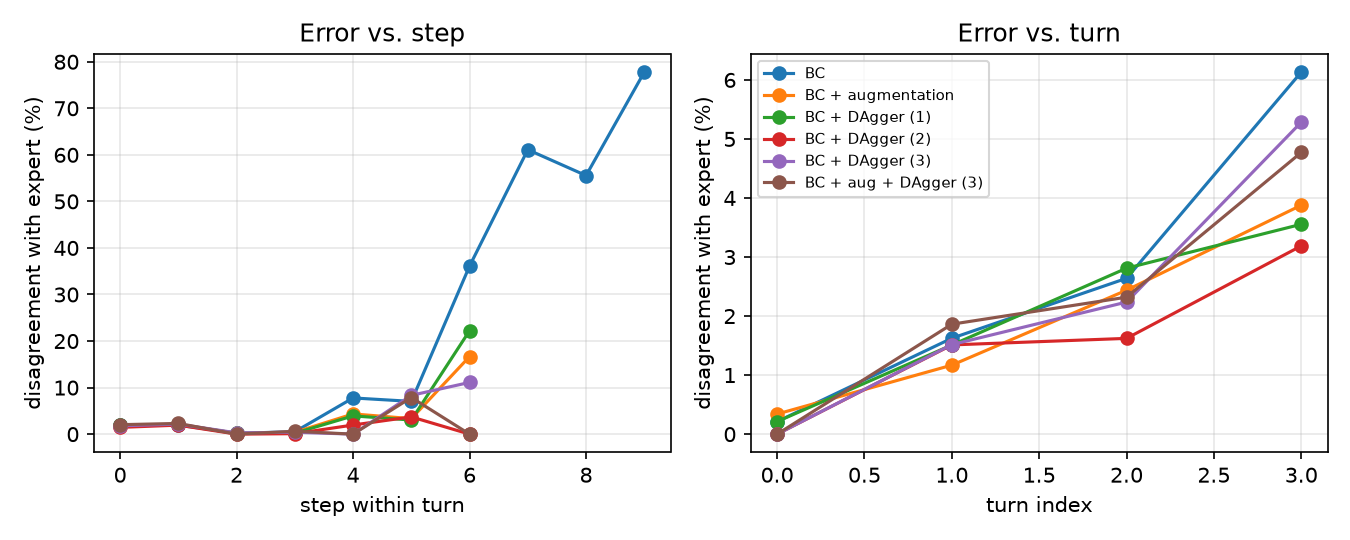
\includegraphics[width=0.8\textwidth]{figures/error_vs_step.png}
\caption{Action disagreement with the scripted expert on policy-visited
states, averaged over three seeds. The left panel groups by zero-indexed
step within a turn. The right panel groups by zero-indexed turn, with
index 3 denoting the fourth turn held out from training. Later steps
include only rollouts that continued that far.}
\label{fig:errorstep}
\end{figure*}

\textbf{Main benchmark (Table~\ref{tab:main}).} All systems shown reach
99.6--100\% revision success. The combined model retains 99.9\% of still-active
constraints, and both rules baselines retain 100\%. The learned variants average
1.16--1.17 excess edits and 0.72 simulated calls per turn. The expert
averages 1.16 excess edits and 0.71 calls. Learned policies use about
14\% fewer simulated calls than cost-aware rules (0.84 calls per turn).
Both always-global controls use 4.19 calls per turn, about $5.8\times$ the
learned policies' cost. Sampled regeneration makes 8.22 excess edits per
scored turn, compared with 1.52 for deterministic regeneration. For BC
with DAgger alone, final pass is 99.6$\pm$0.5, 100.0, and
99.5$\pm$0.3\% after one, two, and three iterations, respectively.

\begin{figure}[tbp]
\centering
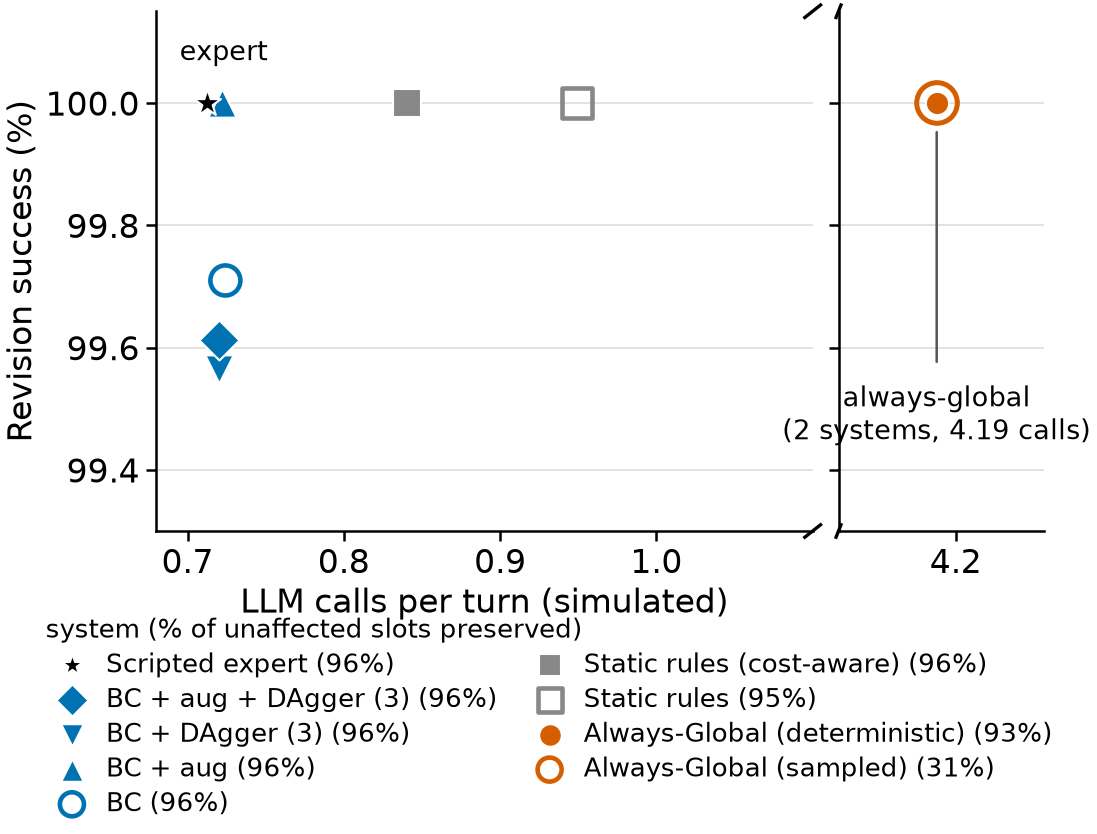
\includegraphics[width=0.92\columnwidth]{figures/pareto.png}
\caption{Revision success versus simulated calls per turn (main test split).
The x-axis is broken at the gap to the always-global controls (4.19 calls).
The y-axis is zoomed near 100\%. The legend reports the share of unaffected
slots preserved. Table~\ref{tab:main} reports edit-optimal preservation.}
\label{fig:pareto}
\end{figure}

\begin{table}[t]
\centering
\caption{Revision success (\%) under a matched cap on simulated calls
per turn.}
\label{tab:capped}
\small
\begin{tabular}{@{}lrr@{}}
\toprule
\textbf{System} & \textbf{Cap 1} & \textbf{Cap 2} \\
\midrule
Static rules & 72.4 & 98.1 \\
Static rules (cost-aware) & 79.7 & 100.0 \\
BC & 97.9 & 99.6 \\
BC + augmentation & 97.8 & 99.8 \\
BC + DAgger (3) & 97.7 & 99.6 \\
BC + aug + DAgger (3) & 97.6 & 99.5 \\
Scripted expert & 98.5 & 100.0 \\
\bottomrule
\end{tabular}
\end{table}

\textbf{Tight call budgets (Table~\ref{tab:capped}).} With one simulated call
per turn, the learned variants in the table reach 97.6--97.9\% revision
success, the scripted expert 98.5\%, cost-aware rules 79.7\%, and plain rules
72.4\%. At two calls, cost-aware rules and the expert reach 100\%, with
learned variants between 99.5 and 99.8\%.

\begin{table*}[t]
\centering
\caption{One-turn budget cuts from an approved itinerary (138 episodes).
The 11 infeasible cuts require clarification. Difficulty for the 127
feasible cuts comes from the scripted expert's bounded repair search.}
\label{tab:multi}
\small
\begin{tabular}{@{}lrrrr@{}}
\toprule
\textbf{System} & \textbf{Success (\%)} & \textbf{Excess edits} &
\textbf{Global rebuilds} & \textbf{Sim.\ calls/turn} \\
\midrule
Always-Global (deterministic) & 100.0 & 4.71 & 100\% & 4.08 \\
Static rules & 100.0 & 5.94 & 75\% & 4.09 \\
Static rules (cost-aware) & 100.0 & 1.03 & 0\% & 2.01 \\
BC & 98.8\,$\pm$\,0.9 & 0.79 & 0\% & 2.06 \\
BC + aug + DAgger (3) & 100.0 & \textbf{0.82} & 0\% & 2.02 \\
Scripted expert & 100.0 & 0.78 & 0\% & 2.01 \\
\bottomrule
\end{tabular}
\end{table*}

\textbf{Multi-component cuts (Table~\ref{tab:multi}).} The original
static rules average 5.94 excess edits and trigger global rebuilds on
75\% of turns. The combined learned coordinator makes about 20\% fewer
excess edits than the cost-aware rules (0.82 vs.\ 1.03), with 100\%
success for both and comparable simulated cost (2.02 vs.\ 2.01 calls).
In the first-seed breakdown, both reach 100\% success at every level.
The combined model and cost-aware rules average 0.13 vs.\ 0.33 excess
edits at one component, 0.41 vs.\ 0.81 at two, and 1.79 each at three.

\textbf{Robustness and compounding error.}
\emph{Forced-mistake recovery}: we inject actions on the first turn of
164 episodes whose original plans need repair. For each local action,
we score recovery on cases it leaves unresolved (116--164 episodes).
Plain BC recovers on 90.5--95.9\% of these cases, BC with three DAgger
iterations on 82.8--100\%, and BC with augmentation on 99.1--100\%.
\emph{Held-out horizons}: in the first-seed breakdown, both BC and
BC+aug+DAgger succeed on 68 of 69 fourth turns (98.6\%). Figure~\ref{fig:errorstep}
reports action disagreement on the trajectories each learned policy visits.
\emph{Clarification}: on infeasible updates, recall is 99.0$\pm$0.4\% for BC
and 100.0\% for BC with augmentation, at 99.5--100\% precision.
Figure~\ref{fig:pareto} summarizes success and simulated cost.

\textbf{Validity and limitations.} The call-count findings depend on the
offline cost model. The global regeneration controls show sensitivity to
plan sampling (30.0\% vs.\ 86.9\% edit-optimal preservation). The
multi-component difficulty labels come from the same bounded scripted
expert used for training, and the alternate wording comes from
handwritten templates. The benchmark covers three-day single-city trips.
For upstream test trips with hidden constraints, we sample starting
budgets and requirements. The evidence for learned dispatch is strongest
at a simulated one-call cap and on excess edits for multi-component cuts.
Under the uncapped protocol, success is comparable at modestly lower
simulated cost. Live evaluation will test these findings with measured
requests and tokens.

\section{Updated plan for the remainder}
\label{sec:plan}

Table~\ref{tab:plan} uses November 30 for the poster/demo session and
December 7 for the final report. Bench handles data and verification,
agents handles planners and LLM integration, learning handles training,
and eval handles metrics, CI, and figures.

\begin{table*}[t]
\centering
\caption{Plan to the final report. Proposed sub-team owners appear in parentheses.}
\label{tab:plan}
\small
\begin{tabular}{@{}>{\raggedright\arraybackslash}p{0.13\textwidth}>{\raggedright\arraybackslash}p{0.79\textwidth}@{}}
\toprule
\textbf{Window} & \textbf{Work} \\
\midrule
Nov 15--22 &
\textbf{H4, live LLM validation} (agents): start with one episode, tune on
validation only, and scale to 30 validation episodes before freezing the
prompts. Log failures and fallbacks and target zero of both for the primary
comparison. \textbf{Single-agent baseline} (agents): return a complete plan
in one request per turn, verify it, and log failures.
\textbf{Freeze test-v2} (bench): prepare non-budget multi-component and
multi-turn revisions on train/validation and freeze the holdout for final
evaluation. \\
Nov 23--29 &
\textbf{Live comparison} (agents + eval): use the same model and frozen
test cases for the single-agent, cost-aware static, and learned systems.
Log requests, tokens, and fallbacks. Apply any live cap to logical requests
end to end, including cache hits. \textbf{Host the app and record the demo}
(agents + eval). \textbf{Prepare and rehearse the poster} (everyone).
Run the LLM-teacher comparison if time permits (learning). \\
Nov 30 & Present the poster and demo (everyone). \\
Dec 1--7 &
\textbf{Final report, contribution statement, and peer evaluation}
(everyone). \textbf{Versioned public release} (bench, reproducibility check
by eval): publish the derived tasks and verifier with a dataset card,
license information, TravelPlanner attribution, and reproduction instructions
by the final submission. \\
\bottomrule
\end{tabular}
\end{table*}

\textbf{Decisions and risks.} If validation stalls, report the offline
comparison as the primary result and document live failures. Check whether
the action mask needs to allow retries with real LLMs. Set a provider
spending cap and distinguish logical requests from billed calls and cache
hits. Flex-TravelPlanner, multi-city trips, paraphrases, and traveler or date
changes are stretch goals after the core comparison. The final report
targets a measured three-system comparison on frozen test cases. The
scripted expert remains an offline reference. The release target is the
derived tasks and verifier by the final submission.

\FloatBarrier
\bibliographystyle{unsrtnat}
\bibliography{references}

\end{document}
